% Chapter 1

\chapter{Introduction} % Main chapter title

\label{Chapter1} % Change X to a consecutive number; for referencing this chapter elsewhere, use \ref{ChapterX}

\lhead{Chapter 1. \emph{Introduction}} % Change X to a consecutive number; this is for the header on each page - perhaps a shortened title

%----------------------------------------------------------------------------------------
%	SECTION 1
%----------------------------------------------------------------------------------------

\section{Preface}\label{section:preface}
This is Section \ref{section:preface} that provides all of the information about my background. Be sure to check out \ref{subsection:postscript} as well for more information. Please find Figure \ref{atrain} for more information.

\subsection{Preface Postscript}\label{subsection:postscript}
Sometimes it is necessary to provide information about the backgrond in segments.

\subsection{Postpostscript}

\begin{figure}[h]
\centering
	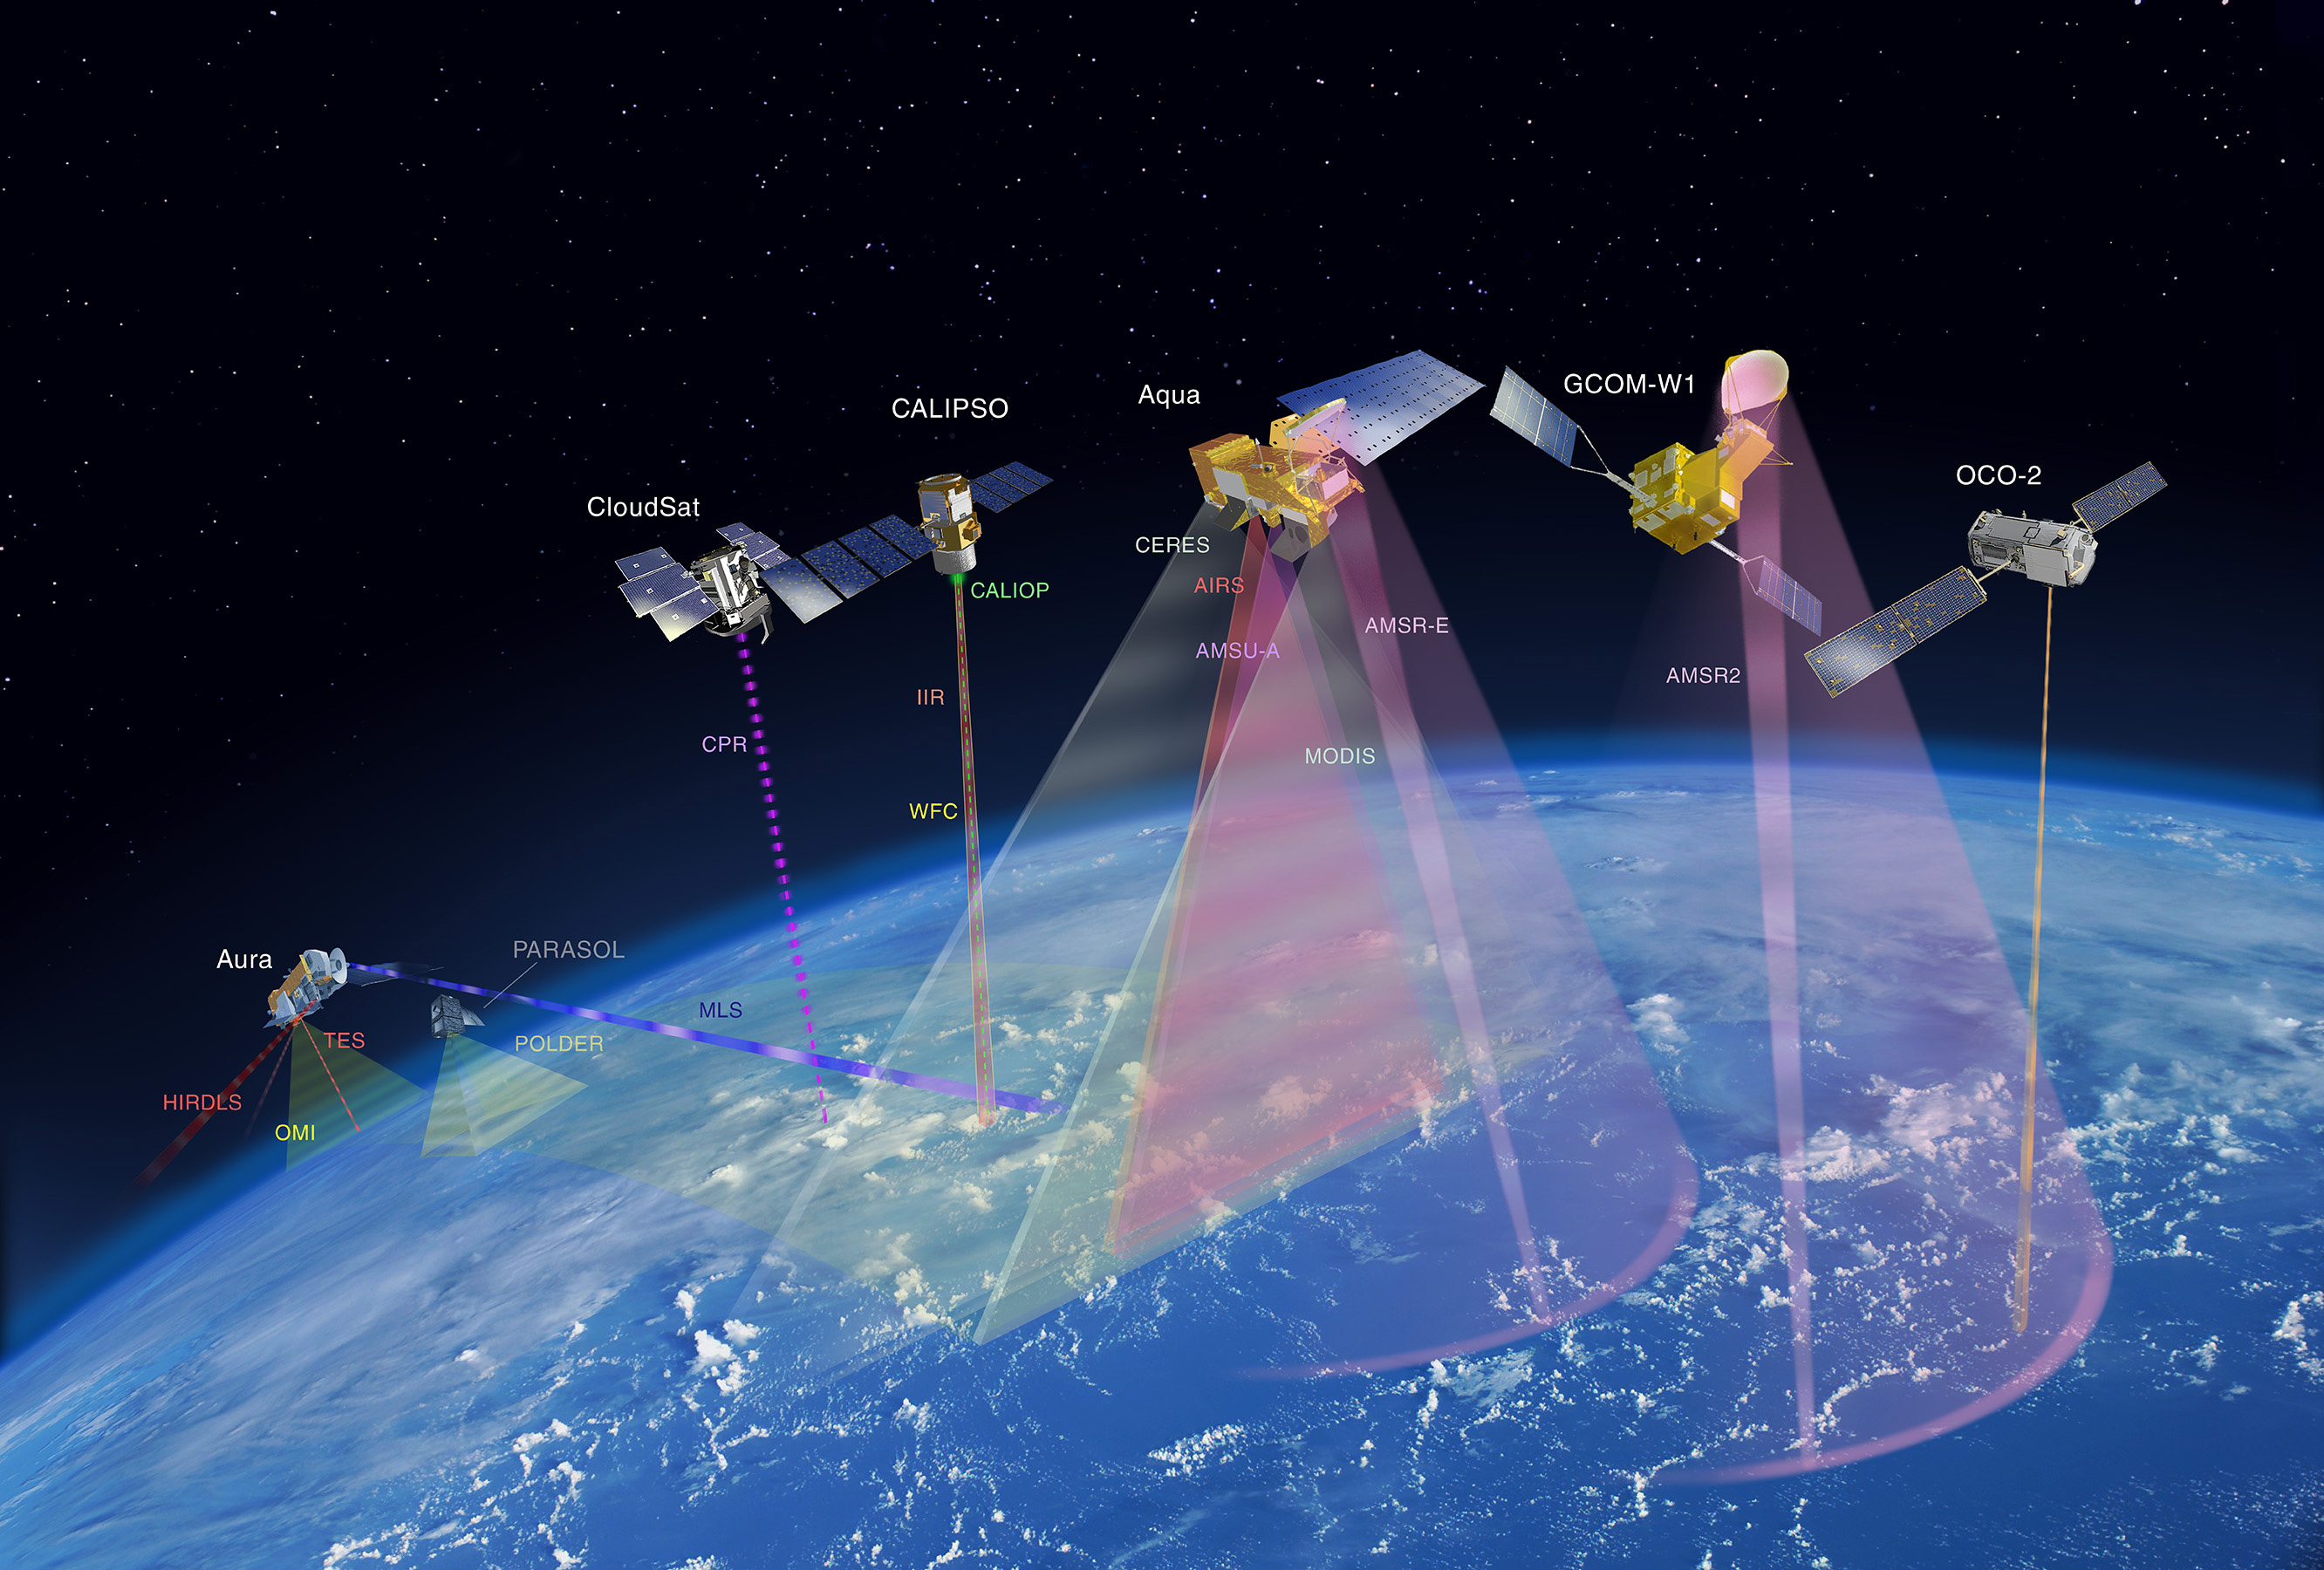
\includegraphics[width=0.6\linewidth]{Figures/atrain.jpeg}
	\rule{35em}{0.5pt}
	\caption[Afternoon Constellation illustration]{An illustration of the Afternoon Constellation (A-Train) satellite mission of NASA with the satellites' respective instruments. CloudSat is second from the left. Illustration courtesy of NASA.}\label{atrain}
\end{figure}

Other areas of interest.

Blah

Blah

\begin{table}[h]
    \centering
    \begin{tabular}{l|l|l}
    ~          & Header 1 & Header 2 \\ \hline \hline
    Category 1 & Data 11  & Data 21  \\ \hline
    Category 2 & Data 12  & Data 22  \\
    \end{tabular}
    \rule{35em}{0.5pt}
    \caption[Short title here.]{We have some data here.}
\end{table}

\begin{itemize}
\item In case you don't know \LaTeX{}
\end{itemize}

\begin{enumerate}
\item \citet{Tanelli2008}
\end{enumerate}